\section{Introdução e objetivos}

\begin{frame}{Introdução}
  \begin{itemize}
    \item O processo de \textbf{Têmpera e Partição}\footnotemark[1] (T\&P) foi inicialmente proposto como rota de tratamento térmico para obtenção de \textbf{microestruturas multifásicas} compostas de martensita e substanciais quantidades de \textbf{austenita enriquecida em carbono}
    \item A \textbf{martensita} ($\alpha'$) confere \textbf{alta resistência}, enquanto \textbf{austenita} ($\gamma$) favorece \textbf{ductilidade} pela ocorrência do fenômeno de transformação martensítica induzida por deformação (TRIP)
  \end{itemize}

  \footnotetext[1]{Speer J, Matlock DK, De Cooman BC, Schroth JG. Acta Mater 2003;51:2611.}
\end{frame}

\begin{frame}{Introdução}
  \begin{itemize}
    \item Têmpera parcial a $Mf < T_T < Ms$ para formar quantidade controlada de $\alpha'$
    \item Reaquecido até $T_P$ para redistribuir C de $\alpha'$ para $\gamma$ (partição)
    \item C diminui Ms de $\gamma$, estabilizando-a a temperatura ambiente
    \item Si e Al adicionados para atrasar precipitação de cementita
  \end{itemize}

  \begin{figure}
    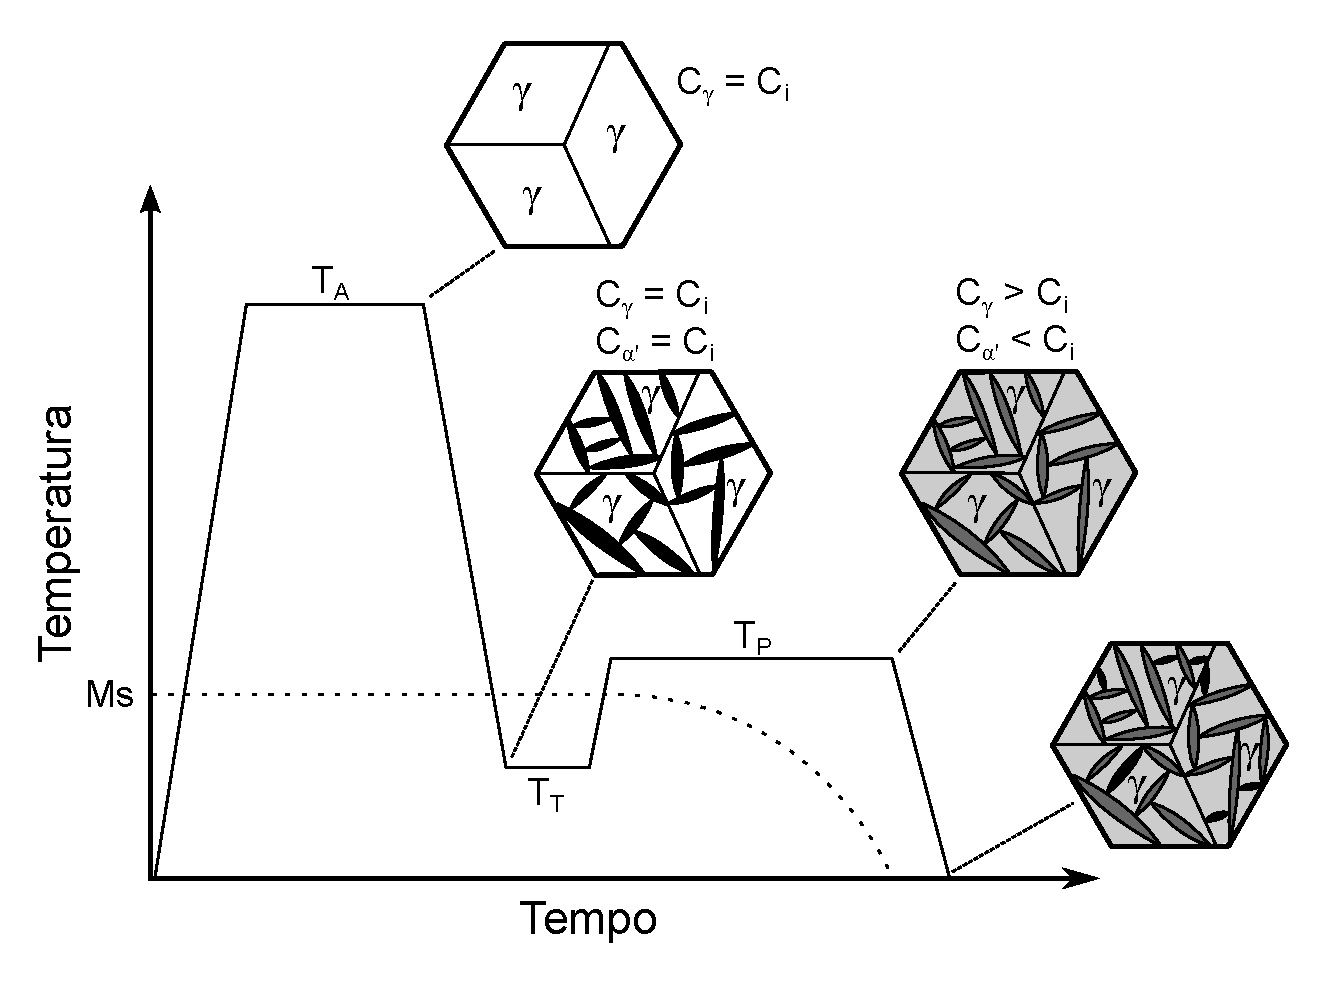
\includegraphics[width=.8\textwidth]{img/Q&P_steel.pdf}
  \end{figure}
\end{frame}

\begin{frame}{Introdução}
  % \only<1>{
  \begin{itemize}
    \item A partição de C de $\alpha'$ para $\gamma$ é termodinamicamente possível devido à diferença de potenciais químicos ($\mu_C^{\alpha'} > \mu_C^\gamma$)
    \item Speer propôs que $\mu_C^{\alpha'}$ e $\mu_C^\gamma$ se igualam após tratamento T\&P
    \item Equilíbrio Constrito de Carbono (ECC): $\mu_C^{\alpha'} = \mu_C^\gamma$  + interface $\alpha'/\gamma$ fixa
    % \item Os teores de C em $\alpha'$ e $\gamma$ são definidos a partir de $\mu_C^{\alpha'} = \mu_C^\gamma$ e das frações iniciais de $\alpha'$ e $\gamma$: Equilíbrio Constrito de Carbono (ECC)
    % \item Assim, C em $\alpha'$ e $\gamma$ depende da fração inicial de $\alpha'$ (depende de $T_T$)
  \end{itemize}

  \begin{figure}
    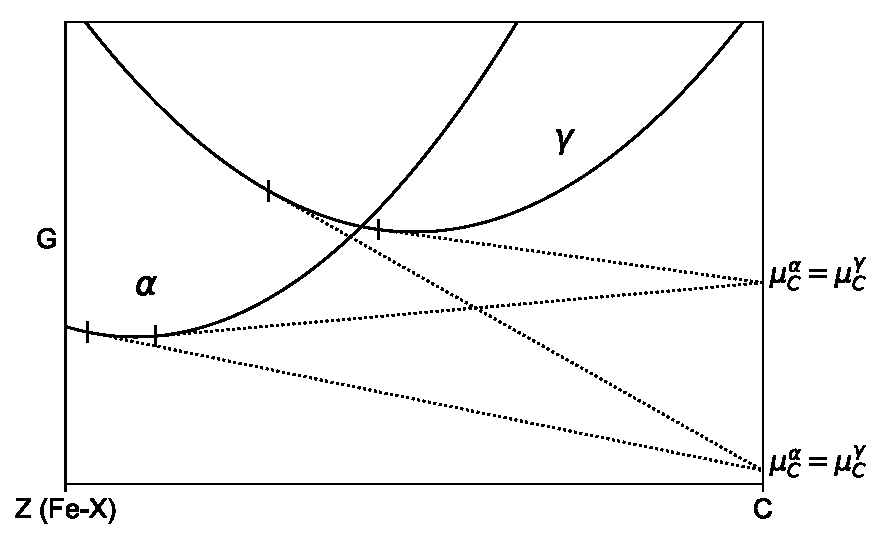
\includegraphics[width=.7\textwidth]{img/common_tangent_CCE.pdf}
  \end{figure}
  % }
  % \only<2>{
  %   \begin{figure}
  %     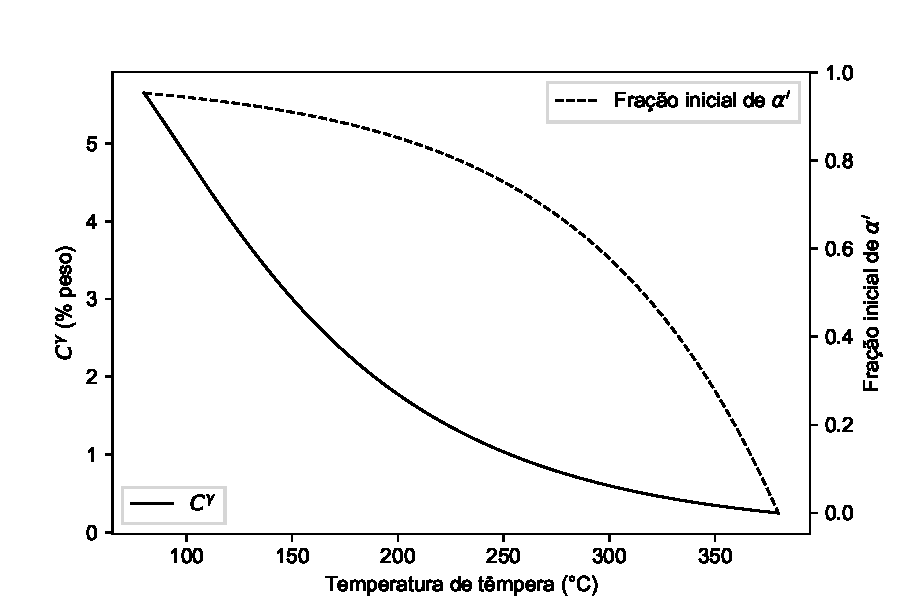
\includegraphics[width=.9\textwidth]{img/CCE_scheme.pdf}
  %   \end{figure}
  % }
\end{frame}

% \begin{frame}
%   \begin{itemize}
%     \item Neste trabalho, a evolução microestrutural e cinética durante a aplicação do processo de \textbf{Têmpera e Partição}\footnotemark[1] (T\&P) de um ferro fundido nodular foi estudada.
%     \item Esta microestrutura promete oferecer propriedades análogas às obtidas durante a transformação bainítica interrompida e aços TRIP e no ferro fundido nodular austemperado (ADI)
%   \end{itemize}
% \end{frame}

%\begin{frame}{Introdução}{Modelo termodinâmico aplicado ao T\&P}
  %\begin{itemize}
    %\item Modelo de Speer (2003): interface $\alpha'$:$\gamma$ imóvel e eq. apenas entre os átomos de C (Equilíbrio Restringido de Carbono - ERC)
    %\item Com base neste modelo, possível determinar \textbf{Temperatura de Têmpera} ótima TO que fornece maior quantidade de austenita
    %\item TT > TO: pouca $\alpha'$ formada, menos carbono para partição para $\gamma$; martensita fresca
    %\item TT < TO: $\gamma$ estabilizado à temperatura ambiente; quantidades menores de $\gamma$ pois é consumido pela formação de $\alpha'$ na têmpera
  %\end{itemize}
%
  %\begin{figure}
  %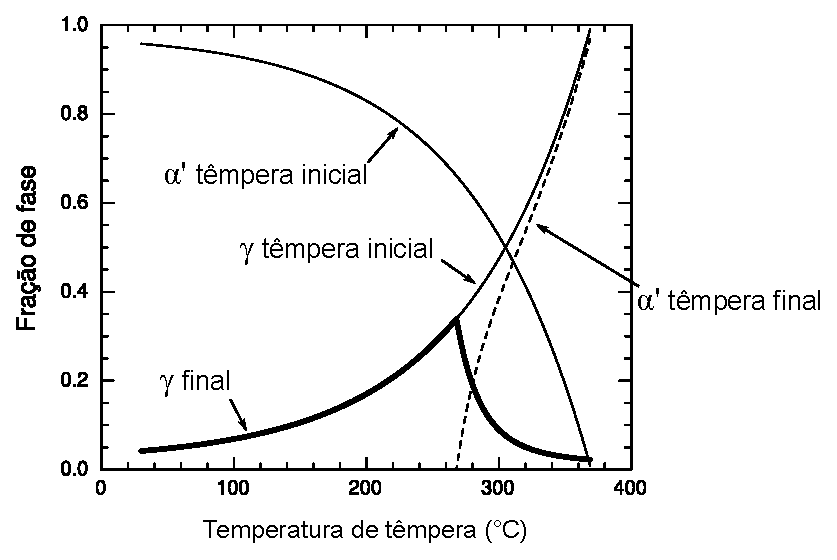
\includegraphics[height=5cm]{../texto/img/TPprevisto.pdf}
  %\end{figure}
%\end{frame}

\begin{frame}{Introdução}
  \begin{block}{Speer, 2004\footnotemark[1]}
    \begin{itemize}
    \item Speer propôs que o elevado teor de Si utilizado na elaboração de ferros fundidos os faria candidatos ótimos para serem submetido à rota T\&P, produzindo microestruturas semelhantes à dos \textbf{ferros fundidos austemperados} (ADI)
    \item Alunos de graduação da Colorado School of Mines, orientados por Speer, submeteram um ferro fundido nodular à rota T\&P e determinaram que o enriquecimento em C de $\gamma$ foi semelhante ao ADI, mas sua retenção foi significativamente menor
    \end{itemize}
  \end{block}

  % \begin{figure}
  % 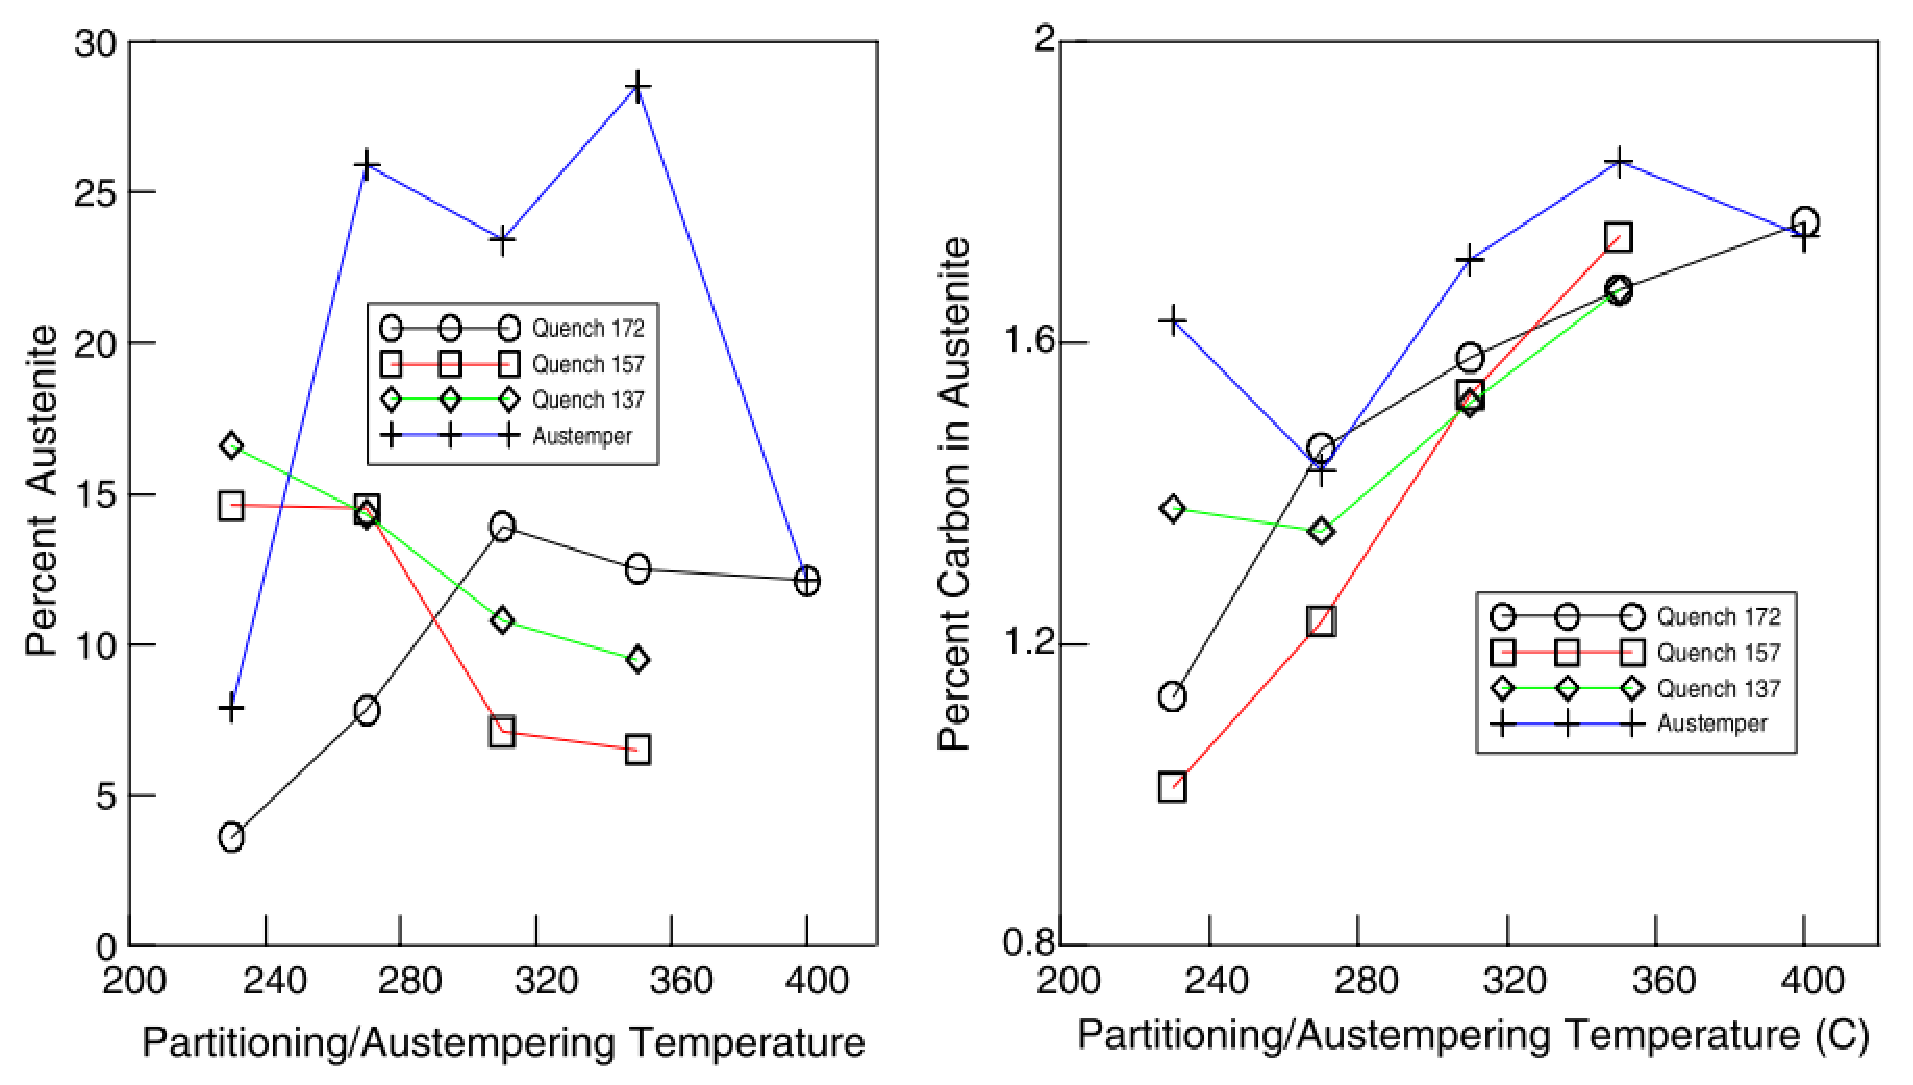
\includegraphics[height=3.8cm]{img/Speer2004.pdf}
  % \end{figure}

  \footnotetext[1]{Speer JG, Edmonds D V., Rizzo FC, Matlock DK. Curr Opin Solid State Mater Sci 2004;8:219.}
\end{frame}

\begin{frame}{Introdução}

  \begin{block}{Dissertação de Anderson J. S. T. Silva\footnotemark[1]}
    \begin{itemize}
    \item Duas ligas comerciais de ferro fundido nodular com alto manganês (> 0,5\%) $\rightarrow$ intensa segregação para contornos de célula eutética
    \item T\&P para diferentes tempos e temperaturas de partição; $T_T$ fixo
    \item Microestrutura composta de $\alpha'$ particionada e grandes quantidades de \textbf{ausferrita} (ferrita bainítica [$\alpha_b$] + $\gamma$), mesmo microconstituinte obtido no ADI
    \item Identificação de \textbf{janela de processo} similar ao ADI, cujo fim é associado ao 2º estágio da reação bainítica
    \end{itemize}

    % \begin{figure}
    %   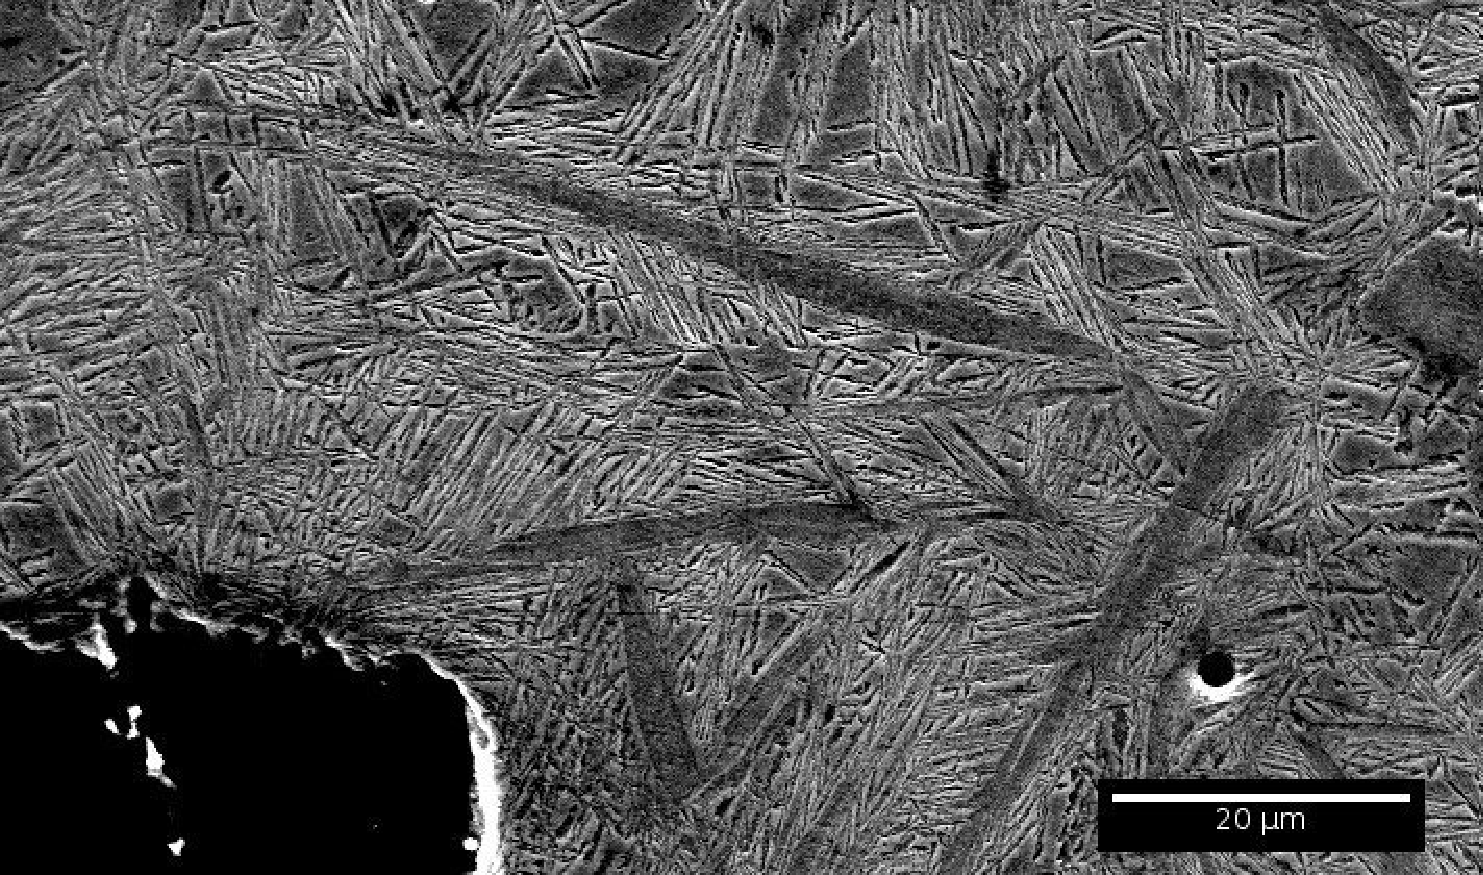
\includegraphics[height=.3\textwidth]{img/MEV_Anderson.pdf}
    % \end{figure}
  \end{block}

  \footnotetext[1]{Silva AJST. Têmpera E Partição de Ferros Fundidos Nodulares. Dissertação (Mestrado). EPUSP, 2013.}
\end{frame}

\begin{frame}{Objetivos}
  Esse trabalho faz parte de um projeto maior que objetiva:
  \begin{enumerate}
    \item Demonstrar a viabilidade da rota T\&P aplicada a ferros fundidos (dissertação de mestrado de Anderson J. S. T. Silva, 2013)
    \item \textbf{Compreender as transformações de fases envolvidas, o entendimento de suas respectivas cinéticas e microestruturas obtidas (presente trabalho)}
    \item Medir as propriedades mecânicas do produto (tese doutorado de André Caetano Melado)
  \end{enumerate}
\end{frame}

% \begin{frame}{Objetivos}
%   \begin{enumerate}
%     \item Avaliar o efeito das variáveis de tratamento térmico na microestrutura final
%     \item Caracterizar a cinética da redistribuição de carbono durante a etapa de partição
%     \item Identificar e caracterizar as reações competitivas que podem ocorrer durante o tratamento de partição, como a reação bainítica e a precipitação de carbonetos
%     \item Avaliar o efeito da microssegregação de elementos de liga, inerente a produtos fundidos, na microestrutura final
%     \item Desenvolver um modelo para a cinética local de redistribuição de carbono durante a etapa de partição, considerando o efeito das reações competitivas.
%   \end{enumerate}
% \end{frame}

% %ADI

% %Equilíbrio Restringido de Carbono
